\documentclass[]{book}
\usepackage{lmodern}
\usepackage{amssymb,amsmath}
\usepackage{ifxetex,ifluatex}
\usepackage{fixltx2e} % provides \textsubscript
\ifnum 0\ifxetex 1\fi\ifluatex 1\fi=0 % if pdftex
  \usepackage[T1]{fontenc}
  \usepackage[utf8]{inputenc}
\else % if luatex or xelatex
  \ifxetex
    \usepackage{mathspec}
  \else
    \usepackage{fontspec}
  \fi
  \defaultfontfeatures{Ligatures=TeX,Scale=MatchLowercase}
\fi
% use upquote if available, for straight quotes in verbatim environments
\IfFileExists{upquote.sty}{\usepackage{upquote}}{}
% use microtype if available
\IfFileExists{microtype.sty}{%
\usepackage{microtype}
\UseMicrotypeSet[protrusion]{basicmath} % disable protrusion for tt fonts
}{}
\usepackage[unicode=true]{hyperref}
\hypersetup{
            pdftitle={SQL for Data Science},
            pdfauthor={Hui Lin},
            pdfborder={0 0 0},
            breaklinks=true}
\urlstyle{same}  % don't use monospace font for urls
\usepackage{natbib}
\bibliographystyle{apalike}
\usepackage{color}
\usepackage{fancyvrb}
\newcommand{\VerbBar}{|}
\newcommand{\VERB}{\Verb[commandchars=\\\{\}]}
\DefineVerbatimEnvironment{Highlighting}{Verbatim}{commandchars=\\\{\}}
% Add ',fontsize=\small' for more characters per line
\usepackage{framed}
\definecolor{shadecolor}{RGB}{248,248,248}
\newenvironment{Shaded}{\begin{snugshade}}{\end{snugshade}}
\newcommand{\KeywordTok}[1]{\textcolor[rgb]{0.13,0.29,0.53}{\textbf{{#1}}}}
\newcommand{\DataTypeTok}[1]{\textcolor[rgb]{0.13,0.29,0.53}{{#1}}}
\newcommand{\DecValTok}[1]{\textcolor[rgb]{0.00,0.00,0.81}{{#1}}}
\newcommand{\BaseNTok}[1]{\textcolor[rgb]{0.00,0.00,0.81}{{#1}}}
\newcommand{\FloatTok}[1]{\textcolor[rgb]{0.00,0.00,0.81}{{#1}}}
\newcommand{\ConstantTok}[1]{\textcolor[rgb]{0.00,0.00,0.00}{{#1}}}
\newcommand{\CharTok}[1]{\textcolor[rgb]{0.31,0.60,0.02}{{#1}}}
\newcommand{\SpecialCharTok}[1]{\textcolor[rgb]{0.00,0.00,0.00}{{#1}}}
\newcommand{\StringTok}[1]{\textcolor[rgb]{0.31,0.60,0.02}{{#1}}}
\newcommand{\VerbatimStringTok}[1]{\textcolor[rgb]{0.31,0.60,0.02}{{#1}}}
\newcommand{\SpecialStringTok}[1]{\textcolor[rgb]{0.31,0.60,0.02}{{#1}}}
\newcommand{\ImportTok}[1]{{#1}}
\newcommand{\CommentTok}[1]{\textcolor[rgb]{0.56,0.35,0.01}{\textit{{#1}}}}
\newcommand{\DocumentationTok}[1]{\textcolor[rgb]{0.56,0.35,0.01}{\textbf{\textit{{#1}}}}}
\newcommand{\AnnotationTok}[1]{\textcolor[rgb]{0.56,0.35,0.01}{\textbf{\textit{{#1}}}}}
\newcommand{\CommentVarTok}[1]{\textcolor[rgb]{0.56,0.35,0.01}{\textbf{\textit{{#1}}}}}
\newcommand{\OtherTok}[1]{\textcolor[rgb]{0.56,0.35,0.01}{{#1}}}
\newcommand{\FunctionTok}[1]{\textcolor[rgb]{0.00,0.00,0.00}{{#1}}}
\newcommand{\VariableTok}[1]{\textcolor[rgb]{0.00,0.00,0.00}{{#1}}}
\newcommand{\ControlFlowTok}[1]{\textcolor[rgb]{0.13,0.29,0.53}{\textbf{{#1}}}}
\newcommand{\OperatorTok}[1]{\textcolor[rgb]{0.81,0.36,0.00}{\textbf{{#1}}}}
\newcommand{\BuiltInTok}[1]{{#1}}
\newcommand{\ExtensionTok}[1]{{#1}}
\newcommand{\PreprocessorTok}[1]{\textcolor[rgb]{0.56,0.35,0.01}{\textit{{#1}}}}
\newcommand{\AttributeTok}[1]{\textcolor[rgb]{0.77,0.63,0.00}{{#1}}}
\newcommand{\RegionMarkerTok}[1]{{#1}}
\newcommand{\InformationTok}[1]{\textcolor[rgb]{0.56,0.35,0.01}{\textbf{\textit{{#1}}}}}
\newcommand{\WarningTok}[1]{\textcolor[rgb]{0.56,0.35,0.01}{\textbf{\textit{{#1}}}}}
\newcommand{\AlertTok}[1]{\textcolor[rgb]{0.94,0.16,0.16}{{#1}}}
\newcommand{\ErrorTok}[1]{\textcolor[rgb]{0.64,0.00,0.00}{\textbf{{#1}}}}
\newcommand{\NormalTok}[1]{{#1}}
\usepackage{longtable,booktabs}
\usepackage{graphicx,grffile}
\makeatletter
\def\maxwidth{\ifdim\Gin@nat@width>\linewidth\linewidth\else\Gin@nat@width\fi}
\def\maxheight{\ifdim\Gin@nat@height>\textheight\textheight\else\Gin@nat@height\fi}
\makeatother
% Scale images if necessary, so that they will not overflow the page
% margins by default, and it is still possible to overwrite the defaults
% using explicit options in \includegraphics[width, height, ...]{}
\setkeys{Gin}{width=\maxwidth,height=\maxheight,keepaspectratio}
\IfFileExists{parskip.sty}{%
\usepackage{parskip}
}{% else
\setlength{\parindent}{0pt}
\setlength{\parskip}{6pt plus 2pt minus 1pt}
}
\setlength{\emergencystretch}{3em}  % prevent overfull lines
\providecommand{\tightlist}{%
  \setlength{\itemsep}{0pt}\setlength{\parskip}{0pt}}
\setcounter{secnumdepth}{5}
% Redefines (sub)paragraphs to behave more like sections
\ifx\paragraph\undefined\else
\let\oldparagraph\paragraph
\renewcommand{\paragraph}[1]{\oldparagraph{#1}\mbox{}}
\fi
\ifx\subparagraph\undefined\else
\let\oldsubparagraph\subparagraph
\renewcommand{\subparagraph}[1]{\oldsubparagraph{#1}\mbox{}}
\fi
\usepackage{booktabs}
\usepackage{longtable}
\usepackage[bf,singlelinecheck=off]{caption}

\setmainfont[UprightFeatures={SmallCapsFont=AlegreyaSC-Regular}]{Alegreya}

\usepackage{framed,color}
\definecolor{shadecolor}{RGB}{248,248,248}

\renewcommand{\textfraction}{0.05}
\renewcommand{\topfraction}{0.8}
\renewcommand{\bottomfraction}{0.8}
\renewcommand{\floatpagefraction}{0.75}

%\renewenvironment{quote}{\begin{VF}}{\end{VF}}
\let\oldhref\href
\renewcommand{\href}[2]{#2\footnote{\url{#1}}}

\ifxetex
  \usepackage{letltxmacro}
  \setlength{\XeTeXLinkMargin}{1pt}
  \LetLtxMacro\SavedIncludeGraphics\includegraphics
  \def\includegraphics#1#{% #1 catches optional stuff (star/opt. arg.)
    \IncludeGraphicsAux{#1}%
  }%
  \newcommand*{\IncludeGraphicsAux}[2]{%
    \XeTeXLinkBox{%
      \SavedIncludeGraphics#1{#2}%
    }%
  }%
\fi

\makeatletter
\newenvironment{kframe}{%
\medskip{}
\setlength{\fboxsep}{.8em}
 \def\at@end@of@kframe{}%
 \ifinner\ifhmode%
  \def\at@end@of@kframe{\end{minipage}}%
  \begin{minipage}{\columnwidth}%
 \fi\fi%
 \def\FrameCommand##1{\hskip\@totalleftmargin \hskip-\fboxsep
 \colorbox{shadecolor}{##1}\hskip-\fboxsep
     % There is no \\@totalrightmargin, so:
     \hskip-\linewidth \hskip-\@totalleftmargin \hskip\columnwidth}%
 \MakeFramed {\advance\hsize-\width
   \@totalleftmargin\z@ \linewidth\hsize
   \@setminipage}}%
 {\par\unskip\endMakeFramed%
 \at@end@of@kframe}
\makeatother

%\renewenvironment{Shaded}{\begin{kframe}}{\end{kframe}}

\newenvironment{rmdblock}[1]
  {
  \begin{itemize}
  \renewcommand{\labelitemi}{
    \raisebox{-.7\height}[0pt][0pt]{
      {\setkeys{Gin}{width=3em,keepaspectratio}\includegraphics{images/#1}}
    }
  }
  \setlength{\fboxsep}{1em}
  \begin{kframe}
  \item
  }
  {
  \end{kframe}
  \end{itemize}
  }
\newenvironment{rmdnote}
  {\begin{rmdblock}{note}}
  {\end{rmdblock}}
\newenvironment{rmdcaution}
  {\begin{rmdblock}{caution}}
  {\end{rmdblock}}
\newenvironment{rmdimportant}
  {\begin{rmdblock}{important}}
  {\end{rmdblock}}
\newenvironment{rmdtip}
  {\begin{rmdblock}{tip}}
  {\end{rmdblock}}
\newenvironment{rmdwarning}
  {\begin{rmdblock}{warning}}
  {\end{rmdblock}}

\usepackage{makeidx}
\makeindex

\urlstyle{tt}

\usepackage{amsthm}
\makeatletter
\def\thm@space@setup{%
  \thm@preskip=8pt plus 2pt minus 4pt
  \thm@postskip=\thm@preskip
}
\makeatother

\frontmatter

\title{SQL for Data Science}
\author{Hui Lin}
\date{2018-01-26}

\usepackage{amsthm}
\newtheorem{theorem}{Theorem}[chapter]
\newtheorem{lemma}{Lemma}[chapter]
\theoremstyle{definition}
\newtheorem{definition}{Definition}[chapter]
\newtheorem{corollary}{Corollary}[chapter]
\newtheorem{proposition}{Proposition}[chapter]
\theoremstyle{definition}
\newtheorem{example}{Example}[chapter]
\theoremstyle{remark}
\newtheorem*{remark}{Remark}
\begin{document}
\maketitle

%\cleardoublepage\newpage\thispagestyle{empty}\null
%\cleardoublepage\newpage\thispagestyle{empty}\null
%\cleardoublepage\newpage
\thispagestyle{empty}
\begin{center}
%\includegraphics{images/dedication.pdf}
\end{center}

\setlength{\abovedisplayskip}{-5pt}
\setlength{\abovedisplayshortskip}{-5pt}

{
\setcounter{tocdepth}{2}
\tableofcontents
}
\chapter*{Statement}\label{statement}


This is my learning notes on SQL. It is initially from Sadie
St.~Lawrence's Coursera course ``SQL for Data Science''.

\mainmatter

\chapter{Getting Started}\label{getting-started}

In this section, you will be able to define SQL and discuss how SQL
differs from other computer languages. You will be able to compare and
contrast the roles of a database administrator and a data scientist, and
explain the differences between one-to-one, one-to-many and many-to-many
relationships with databases. You will be able to use the
\texttt{SELECT} statement and talk about some basic syntax rules. You
will be able to add comments in your code and synthesize its importance.

\textbf{Learning Objectives}

\begin{itemize}
\tightlist
\item
  Distinguish between use of SQL for data science applications and SQL
  for more common data management operations.
\item
  Use an Entity Relationship diagram, describing the data elements,
  their relationships and inter-dependencies and determine if the
  existent data is sufficient to address a business question.
\item
  Identify a subset of data needed from a column or set of columns and
  write and SQL query to limit to those results.
\item
  Create an analysis environment and use \texttt{INSERT} to put data
  into a table
\item
  Add effective comments in your queries so that:

  \begin{enumerate}
  \def\labelenumi{\arabic{enumi}.}
  \tightlist
  \item
    You can remember what you are doing
  \item
    others can review your work
  \end{enumerate}
\end{itemize}

\section{What is SQL?}\label{what-is-sql}

\textbf{S}tructured \textbf{Q}uery \textbf{L}anguage (SQL) is a standard
computer language for relational database management and data
manipulation. SQL is used often to query, insert, update and modify
data. At a basic level, SQL is a way to communicate with database. Many
SQL commands are descriptive words and easy to interpret compared to
many other computer languages. This makes SQL an easy to understand and
learn language.

Another important thing to know about SQL is that it is a non-procedural
language. That means you won't be able to write complete applications
with it. This makes SQL relatively simple but also very powerful
language to interact with data. SQL is all about data and it is used for
three things:

\begin{itemize}
\tightlist
\item
  read and retrieve data from database
\item
  write data into database
\item
  update and insert new data
\end{itemize}

\textbf{Different SQL users}

There are a lot of jobs requre SQL and it is not just for data science.
It is important to understand how different roles might use SQL in their
jobs. The users can be data scientist, programmers, backend developer,
QA engineers, data architects, system engineers and database
administrators (DBA). I want to talk a little more about how DBA use SQL
comparing to data scientist.

\begin{itemize}
\tightlist
\item
  A DBA is responsible for \textbf{managing the entire database and
  guarding it}.
\item
  A data scientist, on the other hand, is typically \textbf{a user of
  that database}.
\end{itemize}

The DBA will be responsible for giving permissions to people and
determining who has access to what data. They are often responsible for
managing the tables and creating them. Data scientist need to get the
rights from DBA to create his/her own table and insert data into them.
The two roles are similar in that they both use SQL to interact with the
data. But the main difference is that the data scientist is really the
end user. Whereas the DBA is the one who administers it, governs it and
manages the database, as a whole.

\begin{longtable}[]{@{}ll@{}}
\toprule
\begin{minipage}[b]{0.22\columnwidth}\raggedright\strut
Database Admin\strut
\end{minipage} & \begin{minipage}[b]{0.22\columnwidth}\raggedright\strut
Data Scientist\strut
\end{minipage}\tabularnewline
\midrule
\endhead
\begin{minipage}[t]{0.22\columnwidth}\raggedright\strut
Manages/governs entire database\strut
\end{minipage} & \begin{minipage}[t]{0.22\columnwidth}\raggedright\strut
End user of a database\strut
\end{minipage}\tabularnewline
\begin{minipage}[t]{0.22\columnwidth}\raggedright\strut
Gives permissions to users\strut
\end{minipage} & \begin{minipage}[t]{0.22\columnwidth}\raggedright\strut
Retrieve data (mainly)\strut
\end{minipage}\tabularnewline
\begin{minipage}[t]{0.22\columnwidth}\raggedright\strut
Determines access to data\strut
\end{minipage} & \begin{minipage}[t]{0.22\columnwidth}\raggedright\strut
May create their own table or test environment\strut
\end{minipage}\tabularnewline
\begin{minipage}[t]{0.22\columnwidth}\raggedright\strut
Manages and creates tables\strut
\end{minipage} & \begin{minipage}[t]{0.22\columnwidth}\raggedright\strut
Combine multiple sources together\strut
\end{minipage}\tabularnewline
\begin{minipage}[t]{0.22\columnwidth}\raggedright\strut
Uses SQL to query and retrive data\strut
\end{minipage} & \begin{minipage}[t]{0.22\columnwidth}\raggedright\strut
Writes complex queries for analysis (maybe but usually not)\strut
\end{minipage}\tabularnewline
\bottomrule
\end{longtable}

\textbf{SQL and Database Management System(DBMS)}

Despite SQL being standardized since 1986, a lot of different
implementations exist. They deviate more or less from each other. You
can think of SQL as the interpreter between you and the database. How
you write some of the syntax for SQL depends on the relational database
management system you are using. Here are some of the popular ones:

\begin{itemize}
\tightlist
\item
  SQL Server
\item
  IBM DB2 Oracle
\item
  Sybase ASE
\item
  PostgreSQL
\item
  MySQL
\item
  Microsoft SQL Server
\item
  Apache Open Office Base
\item
  SQLite
\end{itemize}

In this text, we'll use SQLite. It's important to understand that if you
copy code from this text into another application at work, it may not
work correctly. You should check the type of DBMS you're using and see
if that makes a difference. We will talk about this more when we get to
the syntax later including some of the ways to figure out what those
differences might be.

\begin{quote}
Summary points:

\begin{itemize}
\tightlist
\item
  How you write syntax will depend on what DBMS you are using
\item
  Each DBMS has its own ``dialect''
\item
  SQL can translate
\item
  You will tweak based on the ``dialect'' your DMBS speaks
\end{itemize}
\end{quote}

\chapter{Data Models and Diagrams}\label{data-models-and-diagrams}

\textbf{Learning Objectives}

\begin{itemize}
\tightlist
\item
  Explain why thinking beforing coding is important
\item
  Explain why it is important to understand how the data in a database
  relates to one another
\item
  Describe what a databse is at its core
\item
  Describe data models
\item
  Define relational database system
\item
  Discuss advent of relational databases in SQL
\end{itemize}

\section{Think Before Code}\label{think-before-code}

The reason why thinking beforing coding is importan is because you have
to understand the structure of the data well to effectively write
queries. Understanding your data means the following:

\begin{itemize}
\tightlist
\item
  Understand the business process or subject matter the data is modeled
  after
\item
  Know the business rules
\item
  Understand how your data is organized and structured in the table
\end{itemize}

Before you start to write a query, think about:

\begin{itemize}
\tightlist
\item
  what is the problem you are trying to solve?
\item
  what is the data you need to get?
\item
  how does the data relate to each other?
\item
  how does it interact?
\item
  what are some of the problems that you may want to solve with this
  data and need to be aware of?
\item
  what are the types of joints or business processes in the data
  modeling?
\end{itemize}

This will really help you because not only will you get more accurate
results, but also speed up the time it takes you to work and get things
done. If you start to think about what you're doing before you do it,
you should hopefully also have less rework.

Now what is a database and what is a table?

\begin{quote}
\textbf{Database}: A container (usually a file or set of files) to stre
organized data; a set of related information
\end{quote}

\begin{quote}
\textbf{Tables}: A structured list of data or a specific type
\end{quote}

A database is really a container that is usually a file or set of files
and is used to organize and store all of the data. If you think of this
in real world terms, It'd be like a filing system that has many cabinets
along a wall. Within that system, within a database, we have tables,
these tables are structured lists of data elements or specific data
type. Going back to our analogy, you can think of this as maybe one of
the cabinets within a whole wall of cabinets. Then if we dive further
into the cabinet, into a table, what we find is we have columns and
rows, which of course is what makes up a table. A table is made up of a
series of individual columns, and then a row and a table is a record.
Through tables, rows, and columns, ultimately throughout the database we
have a mechanism to store and retrieve data.

\section{What is Data Model?}\label{what-is-data-model}

Data model is what we use to organize information for multiple tables
and how they relate to each other together. This helps tremendously in
providing structure to the information in the system. Usually a data
model represents a business process and it also helps you understand a
business process. As a data scientist, you often need to work with a
business person in understanding the data and how it fits together. But
at the same time, the business person will learn a lot from the data
modeller to better understand how their business actually works together
by seeing the data and how it interacts with each other.

The data model here is not predictive model which a data scientist often
build. It is a way the tables are represented and organized in a
database. One thing to remember is that a data model should always
represent a real world problem as closely as possible. There are couple
different types of models, and there has been an evolution of data
models.

The evolution of data model traces back to 1960s. There's been
hierarchical, network, relational, entity, relational somatic, and
NoSql.

\begin{figure}[htbp]
\centering
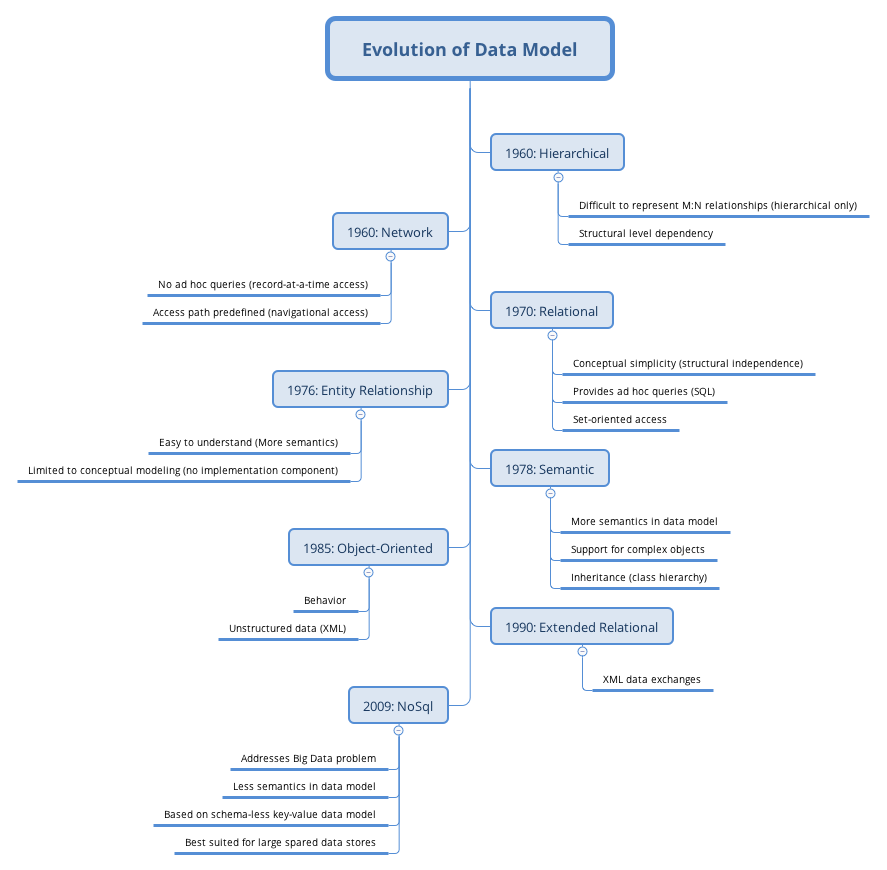
\includegraphics{images/DataModel.png}
\caption{}
\end{figure}

Here we will briefly talk a little about the relational and NoSql.
Because we are going to work a lot with relational model. If you are
interested in learning more, there is material widely available on the
internet and you can do your own research.

The benefits of a relational model are:

\begin{itemize}
\tightlist
\item
  simplify the connections between the data
\item
  allow you to write queries (retrieve/update/write data) easily
\end{itemize}

NoSQL was part of the Big Data movement that you should have already
heard about. It is a mechanism for storage and retrieval where it's not
modeled in a tabular relational format. NoSQL was popular when big data
and unstructured data first came out because you left it unstructured,
but it's now started to soften a little bit, and more commonly referred
to as Not Only SQL. One question to think about: does SQL really have a
role still in the Big Data world, as new things start to come out like
NoSQL and unstructured data?

Next let's talk about the difference between relational and
transactional databases. A \textbf{relational model} is a database
design that shows the relationships between the different tables,
optimizes querying data, makes it easy and intuitive to access the data.
\textbf{Transactional model} is a more operational database. If you are
in healthcare, for example, you may have a transactional database that
is used to store all the claims information and then this information
may not be stored in a great way for querying and using it for analysis.
In fact, you may need to take and extract that transactional information
from the database and move it into a relational model.

Most of what we will be working with is the relational model. There are
3 building blocks for relational model:

\begin{enumerate}
\def\labelenumi{\arabic{enumi}.}
\tightlist
\item
  Entities: a person, place, thing or event. These are very
  distinguishable, unique and distict.
\item
  Attributes: characteristics of this entity.
\item
  Relationships: associations among different entities, can be
  one-to-many, many-to-many and one-to-one.
\end{enumerate}

For example, Pioneer has a great corn seed product called P1197 which
could be an entity. And then we have attributes that are characteristics
of P1197, such as price, average yeilds, units sold, promotion programs.
If you think of a one-to-many relationship, this could be P1197 has many
promotion programs. When you think of a many-to-many relationship, this
could be an example of many products to many different promotion
programs. You may have one product that belongs to different programs or
you may have a program that is available for different products. Then,
if you think of a one-to-one relationship, it could be one product has a
unique price.

To understand these relationships between the tables a lot better,
what's often used to depict this are ER diagrams. ER model is composed
of entity types and specific relationships that can exist between
instances of those entity types. These are usually displayed in a visual
format and a relate represents a \textbf{relationship} between the
tables. It often helps you to understand and represent a
\textbf{business process} and it will show the \textbf{links} between
these tables. The links are important when we join these tables.
\textbf{Being able to look at this diagram and see how they relate to
each other} is really important.

We can use the \textbf{primary key} or \textbf{foreign key} to join
tables. The primary key is a column or set of columns whose values
uniquely identify every row in a table. Foreign key is one or more
columns can be used together to identify a single row in another table.
When we're looking at ER diagrams, which again is one of the ways you
will start to think before you do, you'll look at maybe an ER diagram
and understand what data elements you are trying to join together and
how do you need to get them. But one of the things you need to
understand is how to read this. We talked a little bit about
relationships and the different relationships between a table. There is
a different type of notation that explains the relationships.

\begin{itemize}
\tightlist
\item
  Chen notation
\item
  Crow's foot notation
\item
  UML class diagram notation
\end{itemize}

The Chen notation uses \texttt{1:M} for a one-to-many relationship, and
\texttt{M:N} for a many-to-many relationship and \texttt{1:1} for a
one-to-one relationship.

In Crow's foot notation, we have the train tracks which represent 1 and
then the Crow's foot which represents many.

In UML notation, we have a 1.1 which represents the concept of one and
1.* which represents the concept of many.

\begin{figure}[htbp]
\centering
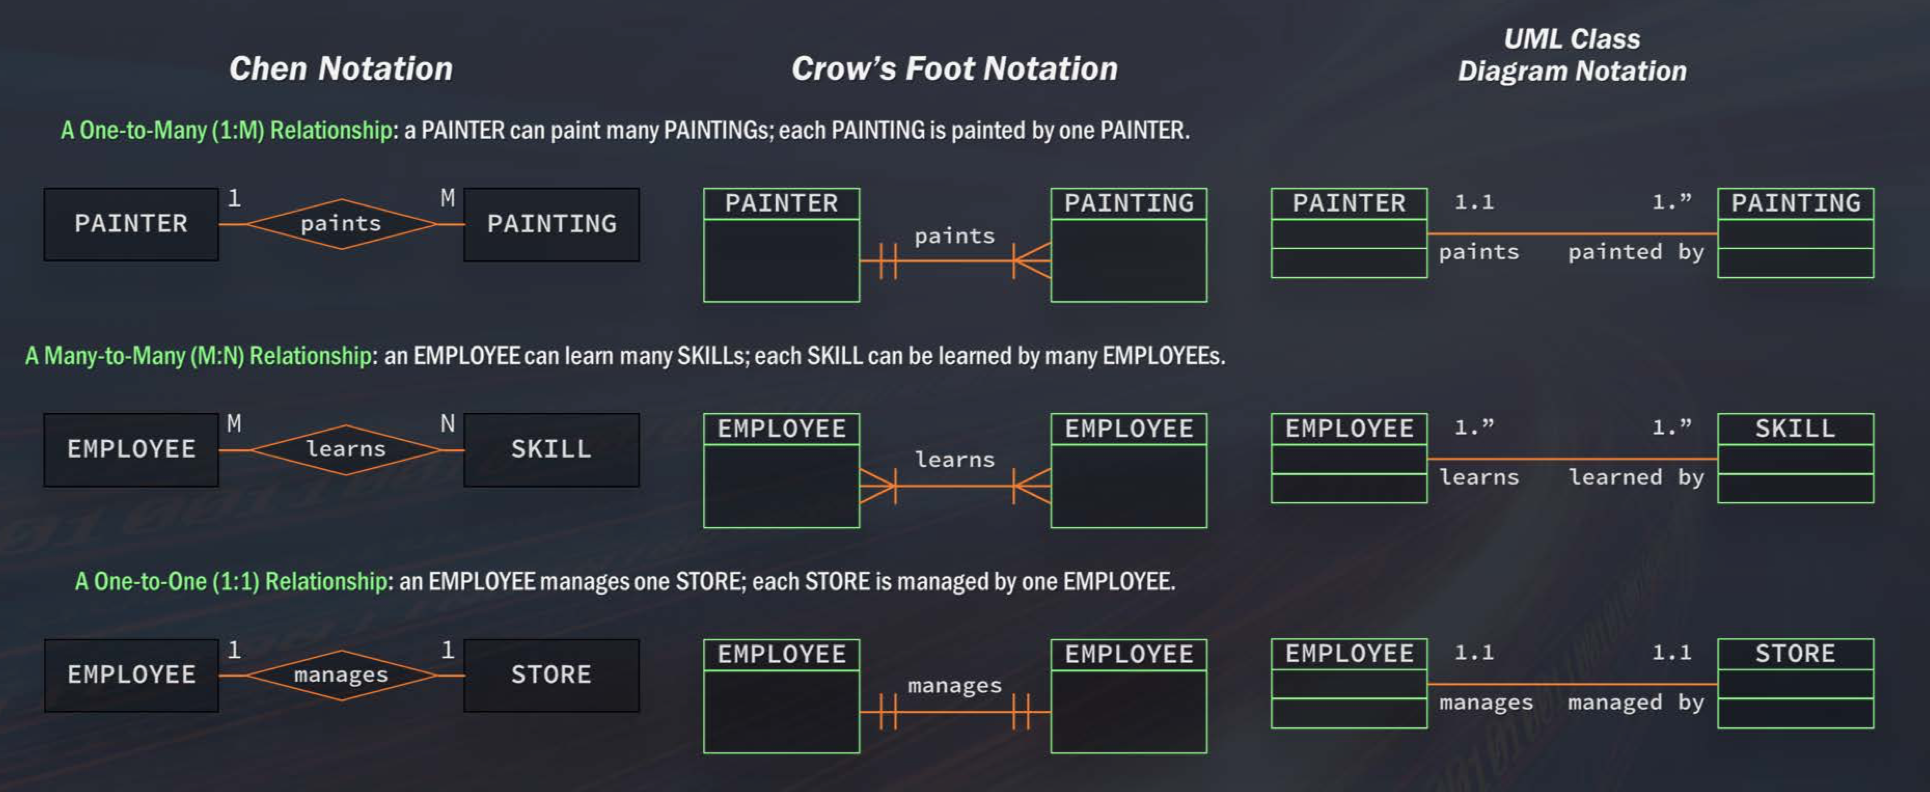
\includegraphics{images/ER.png}
\caption{}
\end{figure}

Get familar with the different notations since you'll be looking at ER
diagrams quite frequently and you'll need to understand these notations
when reading ER diagrams so you can understand how you're going to write
your query and join the table together or even to find out what's listed
in the table. Having a good understanding of why the data is structured
in a particular way and how to read the ER diagrams is necessary for
writing queries and ensuring accurate results.

\section{\texorpdfstring{Retrive Data with
\texttt{SELECT}}{Retrive Data with SELECT}}\label{retrive-data-with-select}

The majority of what data scientists are doing with SQL is retrieving
data. To get started, the first statement to learn is \texttt{SELECT}.
There are two pieces of information to specify in \texttt{SELECT}
statement: what to select and where it is from. It will be
straightforward with an example.

\begin{Shaded}
\begin{Highlighting}[]
\KeywordTok{SELECT} \NormalTok{prod_name}
\KeywordTok{FROM} \NormalTok{Products;}
\end{Highlighting}
\end{Shaded}

\begin{verbatim}
prod_name
Shampoo
Toothpaste
Deodorant
Toothbrush
\end{verbatim}

Ihis example selects product name which a column from the table
(\texttt{prod\_name}). Then you need to specify where to get it from.
Here it is from a table named \texttt{Products}. The output of this is
then going to look like the column listed below. Which it has a column
product name and then all of the list of products. We have shampoo,
toothpaste, deodorant, and toothbrush. If you want to retrieve more than
a single column from a table, then what you need to add the names of the
individual columns separated with a comma:

\begin{Shaded}
\begin{Highlighting}[]
\KeywordTok{SELECT} \NormalTok{prod_name, prod_id, prod_price}
\KeywordTok{FROM} \NormalTok{Products;}
\end{Highlighting}
\end{Shaded}

Request all columns by using the asterisk (\texttt{*}) wildcard
character instead of column names:

\begin{Shaded}
\begin{Highlighting}[]
\KeywordTok{SELECT} \NormalTok{*}
\KeywordTok{FROM} \NormalTok{Products;}
\end{Highlighting}
\end{Shaded}

This is going to go ahead and grab everything from the Products table,
each individual column, and put it into your output.

A lot of times we may want get a view of the table to understand what
data is in there without pulling all the records. In this case, we may
do a ``\texttt{SELECT\ *}''. But if there are 5 million records in it,
we just need a tiny sample of that. In this case, we can use
\texttt{LIMIT} to limit the results.

\begin{Shaded}
\begin{Highlighting}[]
\KeywordTok{SELECT} \NormalTok{prod_name}
\KeywordTok{FROM} \NormalTok{Products}
\KeywordTok{LIMIT} \DecValTok{5}\NormalTok{;}
\end{Highlighting}
\end{Shaded}

Here is an example of how different RDMS differ in syntax:

\begin{figure}[htbp]
\centering
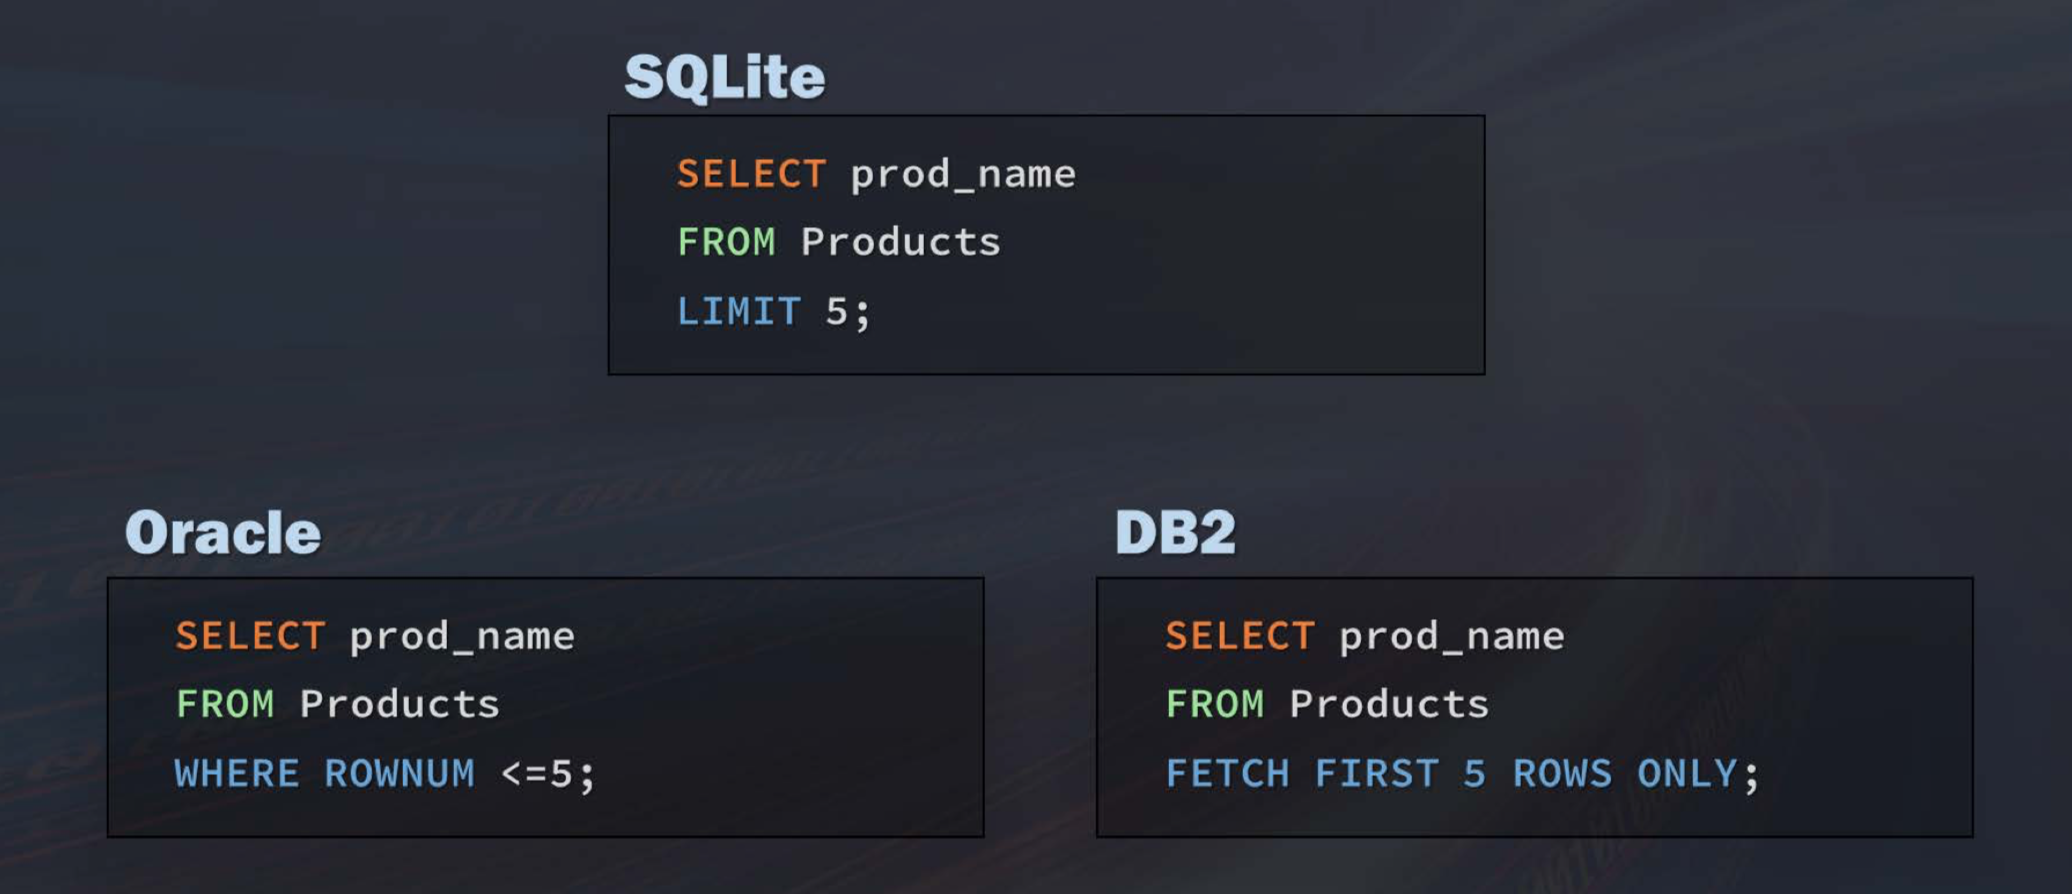
\includegraphics{images/DBMS_diff.png}
\caption{}
\end{figure}

If you are using SQLite and understand it's \texttt{LIMIT\ 5}. When
switch over to a DB2 system, you can easily Google in terms of the
syntax in DB2.

\section{Create Table}\label{create-table}

As a data scientist, you are always building models and making
predictions. You may want to take those predictions that you create and
write them back to a database. This ensures that someone else could then
pick up those predictions and use them in a dashboard. Or you may want
to create a dashboard or visualize it with another tool that can be
hooked up and used with that database. It's also helpful if you're
extracting data off the web or scraping it from somewhere and you want
to store this data in a database. As we have previously discussed, the
data scientist isn't usually the one in charge of managing the entire
database, that usually left to the DBA or some type of administrator.
Even so, it's helpful to have a basic understanding of how this works.
You can use the statement \texttt{CREATE\ TABLE} to do this.

\begin{Shaded}
\begin{Highlighting}[]
\KeywordTok{CREATE} \KeywordTok{TABLE} \NormalTok{Shoes}
\NormalTok{(}
\KeywordTok{Id}     \DataTypeTok{char}\NormalTok{(}\DecValTok{10}\NormalTok{)     }\KeywordTok{PRIMARY} \KeywordTok{KEY}\NormalTok{,}
\NormalTok{Brand  }\DataTypeTok{char}\NormalTok{(}\DecValTok{10}\NormalTok{)     }\KeywordTok{NOT} \KeywordTok{NULL}\NormalTok{,}
\NormalTok{ShoeTypes  }\DataTypeTok{char}\NormalTok{(}\DecValTok{250}\NormalTok{)    }\KeywordTok{NOT} \KeywordTok{NULL}\NormalTok{,}
\NormalTok{Color  }\DataTypeTok{char}\NormalTok{(}\DecValTok{250}\NormalTok{)    }\KeywordTok{NOT} \KeywordTok{NULL}\NormalTok{,}
\NormalTok{Price  }\DataTypeTok{decimal}\NormalTok{(}\DecValTok{8}\NormalTok{,}\DecValTok{2}\NormalTok{) }\KeywordTok{NOT} \KeywordTok{NULL}\NormalTok{,}
\NormalTok{Descp  }\DataTypeTok{Varchar}\NormalTok{(}\DecValTok{750}\NormalTok{) }\KeywordTok{NULL}
\NormalTok{);}
\end{Highlighting}
\end{Shaded}

In the above example, you create a table named ``\texttt{Shoes}'' by
putting the name after \texttt{CREATE\ TABLE}. Then define the list of
columns in the brackets. The first column is \texttt{Id}. It is a
character with lenth 10. And the \texttt{Id} is going to be primary key.
So you define data type (how many characters or decimals you allow to be
inserted into this column), whether or not you allow null values. By
default, it assumes that null values are accepted.

The syntax for creating these tables varies greatly by relational
database management system that you're using. The above example exhibits
the basic structure to create a table. However, it's important to check
the specifications and syntax of the relational database management
system you're using. An important thing to note when creating a table is
to define whether a column can contain a null value or is a primary key.
There are several things to pay special attention here:

\begin{enumerate}
\def\labelenumi{\arabic{enumi}.}
\tightlist
\item
  Don't confuse null value with empty string. Null value is the absence
  of everything, whereas empty string is a value there, such as space.
\item
  A primary key cannot accept null values. The \texttt{Id} in the
  example can never have an empty value or not any value.
\item
  If you indicate that a column cannot be null, then you will get an
  error if there is any missing value in that column.
\end{enumerate}

There are two ways to incert data to the table after defining the
variables:

\begin{enumerate}
\def\labelenumi{(\arabic{enumi})}
\tightlist
\item
  Use \texttt{INSERT\ INTO} statement
\end{enumerate}

\begin{Shaded}
\begin{Highlighting}[]
\KeywordTok{INSERT} \KeywordTok{INTO} \NormalTok{Shoes}
\KeywordTok{VALUES} \NormalTok{( }\StringTok{'14535974'}\NormalTok{,}
\StringTok{'Gucci'}\NormalTok{,}
\StringTok{'Slippers'}\NormalTok{,}
\StringTok{'Pink'}\NormalTok{,}
\StringTok{'695.00'}\NormalTok{,}
\KeywordTok{NULL}
\NormalTok{);}
\end{Highlighting}
\end{Shaded}

The first method will take the first value indicated and put it in the
first column; the second value will go to the second column, and so on
and so forth. It works. However, a potential problem of this method is
that you have no guarantee that data is going into the correct column.
It is better to be more specific.

\begin{enumerate}
\def\labelenumi{(\arabic{enumi})}
\setcounter{enumi}{1}
\tightlist
\item
  Use \texttt{INSERT\ INTO} and \texttt{VALUES}
\end{enumerate}

\begin{Shaded}
\begin{Highlighting}[]
\KeywordTok{INSERT} \KeywordTok{INTO} \NormalTok{Shoes}
\NormalTok{(}\KeywordTok{Id}\NormalTok{, }
\NormalTok{Brand,}
\NormalTok{ShoeTypes,}
\NormalTok{Color,}
\NormalTok{Price,}
\NormalTok{Descp}
\NormalTok{)}
\KeywordTok{VALUES} 
\NormalTok{( }
\StringTok{'14535974'}\NormalTok{,}
\StringTok{'Gucci'}\NormalTok{,}
\StringTok{'Slippers'}\NormalTok{,}
\StringTok{'Pink'}\NormalTok{,}
\StringTok{'695.00'}\NormalTok{,}
\KeywordTok{NULL}
\NormalTok{);}
\end{Highlighting}
\end{Shaded}

The second method also lists the columns. This can be really beneficial
if you want to insert values into some columns but not all. I will
recommend using this method. It's a little safer because you have more
control and know exactly which value is going and into which column.

Now you have learned how to create tables using SQL. Another option is
to create a copy or get a subset of an existing table. A table created
this way is a \textbf{temporary table}. The most important thing to know
about temporary tables is that they will be deleted when the current
client session is terminated. That's why they're called temporary
tables. Why do we need temporary table? Because it is mush faster than
creating a real table. If you have complex queries and you want to
simplify it a bit by creating a subset and then joining to that subset
and driving a new calculation from that, then temporary table is a great
option. You can use the statement \texttt{CREATE\ TEMPORARY\ TABLE} to
do this:

\begin{Shaded}
\begin{Highlighting}[]
\KeywordTok{CREATE} \KeywordTok{TEMPORARY} \KeywordTok{TABLE} \NormalTok{Sandals }\KeywordTok{AS}
\NormalTok{(}
\KeywordTok{SELECT} \NormalTok{*}
\KeywordTok{FROM} \NormalTok{Shoes}
\KeywordTok{WHERE} \NormalTok{ShoeTypes = }\StringTok{'sandals'}
\NormalTok{)}
\end{Highlighting}
\end{Shaded}

In this case, we create a subset of data from \texttt{Shoes} table and
name the new table \texttt{Sandals}. The new table is all records with
shoe type sandals.

\section{SQL Comments}\label{sql-comments}

You may go back to some historical query and modify the query to
retrieve some new data. Comments can help you remember what you were
doing and why. You can also use the comments to mute the expression of
some code, frequently referred to as commenting out code. This technique
helps you troubleshoot some of the issues you have with your query. You
can effectively get rid of parts of your query without actually getting
rid of the statements themselves. And then bring them back in one by one
to see where your query goes awry.

There are two ways of comment.

\begin{enumerate}
\def\labelenumi{(\arabic{enumi})}
\tightlist
\item
  Single line
\end{enumerate}

\begin{Shaded}
\begin{Highlighting}[]
\KeywordTok{SELECT} \KeywordTok{Id}\NormalTok{, }
\CommentTok{-- Brand,}
\NormalTok{ShoeTypes,}
\NormalTok{Color,}
\NormalTok{Price,}
\NormalTok{Descp}
\KeywordTok{FROM} \NormalTok{Shoes}
\end{Highlighting}
\end{Shaded}

The above code uses \texttt{-\/-} to comment out \texttt{Brand,}

\begin{enumerate}
\def\labelenumi{(\arabic{enumi})}
\setcounter{enumi}{1}
\tightlist
\item
  Section
\end{enumerate}

\begin{Shaded}
\begin{Highlighting}[]
\KeywordTok{SELECT} \KeywordTok{Id}\NormalTok{, }
\CommentTok{/* Brand,}
\CommentTok{ShoeTypes,}
\CommentTok{Color, */}
\NormalTok{Price,}
\NormalTok{Descp}
\end{Highlighting}
\end{Shaded}

You can use a combination of a backslash(\texttt{\textbackslash{}}) and
an asterisk(\texttt{*}). What this is effectively saying is, don't run
anything between the two backslashes and the asterisk.

\section{Summary}\label{summary}

In this chapter, we went over many materials. We began by defining SQL.
You should know now that SQL stands for Structured Query Language which
is a standard language to communicate with relational database
management systems (RDMS). You should also know the difference between a
transactional and a relational database. We also introduced important
concept of primary key, foreign key, and table relationship. Make sure
you are familiar with these concepts because we're going to revisit them
a lot in more detail later when we start talking about Joints. We also
discussed some basic SQL Syntax. And you should now be able to write
basic queries statements using \texttt{SELECT} and \texttt{FROM}.
Finally, we wrapped up by going over how to write comments in your code
which are essential to include so that both you and your colleagues can
follow what you were doing and reuse your code. It's a really good habit
to get into as you're starting out. So be sure to keep practicing that
aspect as you begin to write your first query statement.

Here are some resources for further learning:

\begin{itemize}
\tightlist
\item
  \href{https://www.thebalance.com/what-is-sql-and-uses-2071909}{What is
  SQL and How is it Used?}
\item
  \href{https://www.ntchosting.com/encyclopedia/databases/structured-query-language/}{NTC
  Hosting: Structured Query Language}
\item
  \href{https://www.tutorialspoint.com/sqlite/index.htm}{SQLite
  Tutorial}
\item
  \href{http://www.information-management-architect.com/entity-relationship-diagram.html}{Entity
  Relationship Diagram}
\item
  \href{https://www.youtube.com/watch?v=c0_9Y8QAstg}{Norwalk Aberdeen:
  Entity-Relationsip Diagrams (9 Minute YouTube Video)}
\item
  \href{http://www.vertabelo.com/blog/technical-articles/data-warehouse-modeling-star-schema-vs-snowflake-schema}{Star
  Schema vs.~Snowflake Schema}
\item
  \href{https://www.youtube.com/watch?v=KUwOcip7Zzc}{Explain Star Schema
  \& Snow Flake Design (5 Minute YouTube Video)}
\item
  \href{http://www.agiledata.org/essays/dataModeling101.html}{Data
  Modeling 101}
\item
  \href{http://business-analysis-excellence.com/what-is-data-modeling/}{What
  is Data Modeling - An Introduction for Business Analysts}
\item
  \href{https://en.wikipedia.org/wiki/Data_modeling}{Wikipedia: Data
  Modeling}
\end{itemize}

\chapter{Filtering, Sorting, and Calculating Data with
SQL}\label{filtering-sorting-and-calculating-data-with-sql}

\section{Filter}\label{filter}

\subsection{\texorpdfstring{\texttt{WHERE}}{WHERE}}\label{where}

\textbf{Learning Objectives}

\begin{itemize}
\tightlist
\item
  Describe the basics of filtering your data
\item
  Use the \texttt{WHERE} clause with common operators
\item
  Use \texttt{BETWEEN} clause
\item
  Explain the concept of a \texttt{NULL} value
\end{itemize}

Filtering allows us to narrow the data we want to retrieve. Filtering is
also used when you're doing analysis to get very specific about the data
you want to analyze as part of your model. To do this we use what's
called the \texttt{WHERE} clause. And the \texttt{WHERE} clause comes
after \texttt{SELECT} and \texttt{FROM}

\begin{Shaded}
\begin{Highlighting}[]
\KeywordTok{SELECT} \NormalTok{column_name, column_name}
\KeywordTok{FROM} \NormalTok{table_name}
\KeywordTok{WHERE} \NormalTok{column_name }\KeywordTok{operator} \FunctionTok{value}\NormalTok{;}
\end{Highlighting}
\end{Shaded}

Here is a table of common operators:

\begin{longtable}[]{@{}ll@{}}
\toprule
\begin{minipage}[b]{0.13\columnwidth}\raggedright\strut
Operator\strut
\end{minipage} & \begin{minipage}[b]{0.18\columnwidth}\raggedright\strut
Description\strut
\end{minipage}\tabularnewline
\midrule
\endhead
\begin{minipage}[t]{0.13\columnwidth}\raggedright\strut
\texttt{=}\strut
\end{minipage} & \begin{minipage}[t]{0.18\columnwidth}\raggedright\strut
Equal\strut
\end{minipage}\tabularnewline
\begin{minipage}[t]{0.13\columnwidth}\raggedright\strut
\texttt{\textless{}\textgreater{}}\strut
\end{minipage} & \begin{minipage}[t]{0.18\columnwidth}\raggedright\strut
Not equal. Note: In some versions of SQL this operator may be written as
\texttt{!=}\strut
\end{minipage}\tabularnewline
\begin{minipage}[t]{0.13\columnwidth}\raggedright\strut
\texttt{\textgreater{}}\strut
\end{minipage} & \begin{minipage}[t]{0.18\columnwidth}\raggedright\strut
Greater than\strut
\end{minipage}\tabularnewline
\begin{minipage}[t]{0.13\columnwidth}\raggedright\strut
\texttt{\textless{}}\strut
\end{minipage} & \begin{minipage}[t]{0.18\columnwidth}\raggedright\strut
Less than\strut
\end{minipage}\tabularnewline
\begin{minipage}[t]{0.13\columnwidth}\raggedright\strut
\texttt{\textgreater{}=}\strut
\end{minipage} & \begin{minipage}[t]{0.18\columnwidth}\raggedright\strut
Greater than or equal\strut
\end{minipage}\tabularnewline
\begin{minipage}[t]{0.13\columnwidth}\raggedright\strut
\texttt{\textless{}=}\strut
\end{minipage} & \begin{minipage}[t]{0.18\columnwidth}\raggedright\strut
Less than or equal\strut
\end{minipage}\tabularnewline
\begin{minipage}[t]{0.13\columnwidth}\raggedright\strut
BETWEEN\strut
\end{minipage} & \begin{minipage}[t]{0.18\columnwidth}\raggedright\strut
Between an inclusive range\strut
\end{minipage}\tabularnewline
\begin{minipage}[t]{0.13\columnwidth}\raggedright\strut
IS NULL\strut
\end{minipage} & \begin{minipage}[t]{0.18\columnwidth}\raggedright\strut
Is a null value\strut
\end{minipage}\tabularnewline
\bottomrule
\end{longtable}

Let's look at some examples.

\begin{Shaded}
\begin{Highlighting}[]
\KeywordTok{SELECT} \NormalTok{ProductName,}
\NormalTok{UnitPrice,}
\NormalTok{SupplierID}
\KeywordTok{FROM} \NormalTok{Products}
\KeywordTok{WHERE} \NormalTok{ProductName = }\StringTok{'Tofu'}\NormalTok{;}
\end{Highlighting}
\end{Shaded}

In the above example, we filter on a single condition. We look at
ProductName, UnitPrice and SupplierID for tofu. You can similarly look
at products whose prices are greater than or equal to 75.

\begin{Shaded}
\begin{Highlighting}[]
\KeywordTok{SELECT} \NormalTok{ProductName,}
\NormalTok{UnitPrice,}
\NormalTok{SupplierID}
\KeywordTok{FROM} \NormalTok{Products}
\KeywordTok{WHERE} \NormalTok{UnitPrice >= }\DecValTok{75}\NormalTok{;}
\end{Highlighting}
\end{Shaded}

Or you can filter out all records except one value:

\begin{Shaded}
\begin{Highlighting}[]
\KeywordTok{SELECT} \NormalTok{ProductName,}
\NormalTok{UnitPrice,}
\NormalTok{SupplierID}
\KeywordTok{FROM} \NormalTok{Products}
\KeywordTok{WHERE} \NormalTok{ProductName <> }\StringTok{'Tofu'}\NormalTok{;}
\end{Highlighting}
\end{Shaded}

You can filter for a range of values:

\begin{Shaded}
\begin{Highlighting}[]
\KeywordTok{SELECT} \NormalTok{ProductName,}
\NormalTok{Unitprice,}
\NormalTok{SupplierID,}
\NormalTok{UnitsInStock,}
\KeywordTok{FROM} \NormalTok{Products}
\KeywordTok{WHERE} \NormalTok{UnitsInStock }\KeywordTok{BETWEEN} \DecValTok{15} \KeywordTok{AND} \DecValTok{80}\NormalTok{;}
\end{Highlighting}
\end{Shaded}

You can filter \texttt{NULL} values by \texttt{IS\ NULL}

\begin{Shaded}
\begin{Highlighting}[]
\KeywordTok{SELECT} \NormalTok{ProductName,}
\NormalTok{UnitPrice,}
\NormalTok{SupplierID,}
\NormalTok{UnitsInStock}
\KeywordTok{FROM} \NormalTok{Products}
\KeywordTok{WHERE} \NormalTok{ProductName }\KeywordTok{IS} \KeywordTok{NULL}\NormalTok{;}
\end{Highlighting}
\end{Shaded}

\subsection{\texorpdfstring{\texttt{IN}, \texttt{OR} and
\texttt{NOT}}{IN, OR and NOT}}\label{in-or-and-not}

\textbf{Learning Objectives}

\begin{itemize}
\tightlist
\item
  Use the \texttt{IN} and \texttt{OR} operators to filter your data and
  get results you want
\item
  Differentiate between use of the \texttt{IN} and \texttt{BETWEEN}
  operators
\item
  Discuss importance of order of operations
\item
  Explain how and when to use the \texttt{NOT} operator
\end{itemize}

Let's start from\texttt{IN}. To use the IN operator, we need to specify
a range of conditions or a set of values.

\begin{Shaded}
\begin{Highlighting}[]
\KeywordTok{SELECT}
\NormalTok{ProductID,}
\NormalTok{UnitPrice,}
\NormalTok{SupplierID}
\KeywordTok{FROM} \NormalTok{Products}
\KeywordTok{WHERE} \NormalTok{SupplierID }\KeywordTok{IN} \NormalTok{(}\DecValTok{9}\NormalTok{, }\DecValTok{10}\NormalTok{, }\DecValTok{11}\NormalTok{);}
\end{Highlighting}
\end{Shaded}

Another operator is the \texttt{OR} operator. An important thing to know
about this is that a database management system will not evaluate the
second condition in a \texttt{WHERE} clause if the first condition is
met.

\begin{Shaded}
\begin{Highlighting}[]
\KeywordTok{SELECT}
\NormalTok{ProductName,}
\NormalTok{ProductID,}
\NormalTok{UnitPrice,}
\NormalTok{SupplierID,}
\NormalTok{ProductName}
\KeywordTok{FROM} \NormalTok{Products}
\KeywordTok{WHERE} \NormalTok{ProductName = }\StringTok{'Tofu'} \KeywordTok{OR} \StringTok{'Konbu'}\NormalTok{;}
\end{Highlighting}
\end{Shaded}

You can use \texttt{OR} with \texttt{AND}. There is somthing you need to
pay extra attention. Look at the following two examples:

\begin{itemize}
\tightlist
\item
  Example1:
\end{itemize}

\begin{Shaded}
\begin{Highlighting}[]
\KeywordTok{SELECT}
\NormalTok{ProductID,}
\NormalTok{UnitPrice,}
\NormalTok{SupplierID,}
\KeywordTok{FROM} \NormalTok{Products}
\KeywordTok{WHERE} \NormalTok{SupplierID = }\DecValTok{9} \KeywordTok{OR}
\NormalTok{SupplierID = }\DecValTok{11}
\KeywordTok{AND} \NormalTok{UnitPrice > }\DecValTok{15}\NormalTok{;}
\end{Highlighting}
\end{Shaded}

\begin{figure}[htbp]
\centering
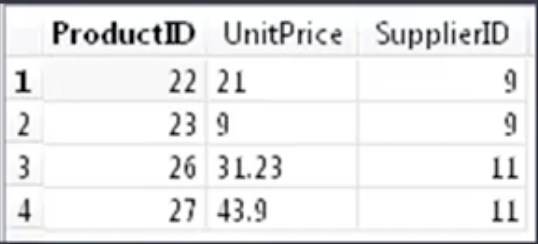
\includegraphics[width=0.40000\textwidth]{images/ex1.png}
\caption{}
\end{figure}

\begin{itemize}
\tightlist
\item
  Example2:
\end{itemize}

\begin{Shaded}
\begin{Highlighting}[]
\KeywordTok{SELECT}
\NormalTok{ProductID,}
\NormalTok{UnitPrice,}
\NormalTok{SupplierID}
\KeywordTok{FROM} \NormalTok{Products}
\KeywordTok{WHERE} \NormalTok{(SupplierID = }\DecValTok{9} \KeywordTok{OR}
\NormalTok{SupplierID = }\DecValTok{11}\NormalTok{)}
\KeywordTok{AND} \NormalTok{UnitPrice > }\DecValTok{15}\NormalTok{;}
\end{Highlighting}
\end{Shaded}

\begin{figure}[htbp]
\centering
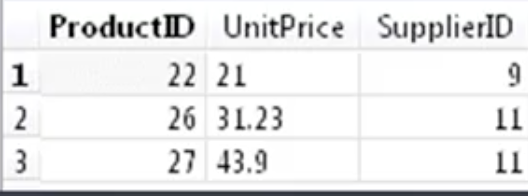
\includegraphics[width=0.40000\textwidth]{images/ex2.png}
\caption{}
\end{figure}

Since SQL processes the \texttt{OR} before the \texttt{AND}, in
example1, SQL will stop after processing \texttt{OR}, so it won't even
get to the operation after \texttt{AND}. In order to solve that, you
need to use parentheses.

Even you don't have to use a parenthesis, but it's always really
recommended. This way you're not relying on the default order of
operations.

You can use \texttt{NOT} to get the supplementary part:

\begin{Shaded}
\begin{Highlighting}[]
\KeywordTok{SELECT} \NormalTok{*}
\KeywordTok{FROM} \NormalTok{Employees}
\KeywordTok{WHERE} \KeywordTok{NOT} \NormalTok{City=}\StringTok{'London'} \KeywordTok{AND}
\KeywordTok{NOT} \NormalTok{City=}\StringTok{'Seattle'}\NormalTok{;}
\end{Highlighting}
\end{Shaded}

\textbf{Wildcards}

Have you ever come across data where you knew either the beginning or
end of something, but didn't know the rest of it? Or maybe you know that
something is like something else, but slightly different. In the rest of
this section, we are going to discuss the use of the wildcards and the
\texttt{LIKE} operator. You will learn the concept of wildcards,
including their advantages and disadvantages.

Wildcard is a really powerful especially for string values or text data.
A wildcard is a special character used to match parts of a value. You
search for a pattern of string. \texttt{LIKE} works for both string and
numerical variables. But wildcards cannot be used for numerical data.

\textbf{\texttt{\%} Wildcards}

\begin{longtable}[]{@{}ll@{}}
\toprule
Wildcard & Action\tabularnewline
\midrule
\endhead
\texttt{\%carrot} & Grab anything ending with the word
\texttt{carrot}\tabularnewline
\texttt{carrot\%} & Grab anything after the word
\texttt{carrot}\tabularnewline
\texttt{\%carrot\%} & Grab anything containing the word
\texttt{carrot}\tabularnewline
\texttt{today\%happy} & Grab anything that starts with \texttt{today}
and ends with \texttt{happy}\tabularnewline
\texttt{t\%@gmail.com} & Grab gmail address that start with
\texttt{t}\tabularnewline
\bottomrule
\end{longtable}

Underscore(\texttt{\_}) wildcard matches a single character but it is
not supported by DB2.

\begin{Shaded}
\begin{Highlighting}[]
\KeywordTok{WHERE} \KeywordTok{size} \KeywordTok{LIKE} \NormalTok{`_carrot`}
\end{Highlighting}
\end{Shaded}

Output:

\begin{verbatim}
lcarrot
mcarrot
scarrot
\end{verbatim}

It is identical with:

\begin{Shaded}
\begin{Highlighting}[]
\KeywordTok{WHERE} \KeywordTok{size} \KeywordTok{LIKE} \NormalTok{`%carrot`}
\end{Highlighting}
\end{Shaded}

Bracket (\texttt{{[}{]}}) wildcard specifies a set of characters in a
specific location. It does not work with all DBMS. It does not work with
SQLite.

There are some downsides to using wildcards:

\begin{itemize}
\tightlist
\item
  Takes longer to run
\item
  Better to use another operator (if possible)
  \texttt{=},\texttt{\textless{}},\texttt{\textgreater{}=} etc.
\item
  Depending on the system
\item
  Hard to read
\end{itemize}

\section{Sort}\label{sort}

\textbf{Learning Objectives}

\begin{itemize}
\tightlist
\item
  Explain some of the rules related to using the \texttt{ORDER\ BY}
  clause
\item
  Use the \texttt{ORDER\ BY} clause to sort data either in ascending or
  descending order
\end{itemize}

\texttt{ORDER\ BY} allows us to sort data by particular columns. Now
there are a few rules when using \texttt{ORDER\ BY}:

\begin{enumerate}
\def\labelenumi{\arabic{enumi}.}
\tightlist
\item
  It can take multiple column names.
\item
  If you're doing multiple columns, you just want to make sure you're
  adding a comma after that.
\item
  You can sort by a column that you didn't retrieve.
\item
  It must always be the last clause in the select statement.
\end{enumerate}

You can sort by column position. For example, sort by column 2 and 3:

\begin{Shaded}
\begin{Highlighting}[]
\KeywordTok{ORDER} \KeywordTok{BY} \DecValTok{2}\NormalTok{,}\DecValTok{3}
\end{Highlighting}
\end{Shaded}

There are also some directions as with any type of sorting, either in
ascending, \texttt{ASC}, or descending order, \texttt{DESC}. This is
only applied to the column name it directly proceeds. If you're using
order by descending and have unit price, it's not going to do it for all
of columns after the \texttt{DESC}. You have to specify each individual
columns for ascending and descending, if you want it that way.

\section{Math Operations}\label{math-operations}

\textbf{Learning Objectives}

\begin{itemize}
\tightlist
\item
  perform basic math calculations
\item
  discuss in more detail the concept and the order of operations
\item
  describe what can be done in terms of analysis by using math operators
  and SQL with math calculations
\end{itemize}

Let's start with some simple ones. We have the addition, subtraction,
multiplication, and division.

\begin{Shaded}
\begin{Highlighting}[]
\KeywordTok{SELECT} 
\NormalTok{ProductID,}
\NormalTok{UnitsOnOrder,}
\NormalTok{UnitPrice,}
\NormalTok{UnitsOnOrder * UnitPrice }\KeywordTok{AS} \NormalTok{Total_Order_Cost}
\KeywordTok{FROM} \NormalTok{Products}
\end{Highlighting}
\end{Shaded}

In this example, we get the total order cost by multiplying units on
order with unit price. And then, we name the new column
\texttt{Total\_Order\_Cost} by using \texttt{AS}.

You dont't have to \texttt{SELECT} the unit price and the units on the
order to calculate the total cost. You could have just selected the
product ID and then calculated the new field. But it is a nice thing to
make sure it all adds up and looks right.

Now let's add these operators together. Just as any math you're doing,
it's going to follow normal order of operations. You probably remember
the order of operations from past math classes. Operations in
parentheses are handled first, then power, multiplication, division,
addition, and subtraction.

\begin{Shaded}
\begin{Highlighting}[]
\KeywordTok{SELECT}
\NormalTok{ProductID,}
\NormalTok{Quantity,}
\NormalTok{UnitPrice,}
\NormalTok{Discount,}
\NormalTok{(UnitPrice - Discount)/Quantity }\KeywordTok{AS} \NormalTok{Total_Cost}
\KeywordTok{FROM} \NormalTok{Products}
\end{Highlighting}
\end{Shaded}

\section{Aggregrate Functions}\label{aggregrate-functions}

\textbf{Learning Objectives}

\begin{itemize}
\tightlist
\item
  Describe various aggregate functions
\item
  Use various aggregate functions: \texttt{AVERAGE}, \texttt{COUNT},
  \texttt{MIN}, \texttt{MAX} and \texttt{SUM} to summarize and analyze
  data
\item
  Describe the \texttt{DISTINCT} function
\end{itemize}

Aggregate functions are used for various things such as finding the
highest or lowest values, total number of records, average value, etc.
We're going to use a lot of these different types of aggregate functions
to get descriptive statistics. The aggregate functions we can use are
\texttt{AVG}, \texttt{COUNT}, \texttt{MIN}, \texttt{MAX}, and
\texttt{SUM} and all of these are pretty self explanatory.

\begin{longtable}[]{@{}ll@{}}
\toprule
Function & Description\tabularnewline
\midrule
\endhead
\texttt{AVG()} & Averages a column of values\tabularnewline
\texttt{COUNT()} & Counts the number of values\tabularnewline
\texttt{MIN()} & Finds the minimum value\tabularnewline
\texttt{MAX()} & Finds the maximum value\tabularnewline
\texttt{SUM()} & Sums the column values\tabularnewline
\bottomrule
\end{longtable}

\begin{itemize}
\tightlist
\item
  \texttt{AVG()}
\end{itemize}

\begin{Shaded}
\begin{Highlighting}[]
\KeywordTok{SELECT} \FunctionTok{AVG}\NormalTok{(UnitPrice) }\KeywordTok{AS} \NormalTok{avg_price}
\KeywordTok{FROM} \NormalTok{Products;}
\end{Highlighting}
\end{Shaded}

\begin{itemize}
\tightlist
\item
  \texttt{COUNT(*)}: Counts all the rows in a table containing
  \texttt{NULL} values
\end{itemize}

\begin{Shaded}
\begin{Highlighting}[]
\KeywordTok{SELECT} \FunctionTok{COUNT}\NormalTok{(*) }\KeywordTok{AS} \NormalTok{total_customers}
\KeywordTok{FROM} \NormalTok{Customers;}
\end{Highlighting}
\end{Shaded}

\begin{itemize}
\tightlist
\item
  \texttt{COUNT(column)}: Counts all the rows in a specific column
  ignoring \texttt{NULL} values
\end{itemize}

\begin{Shaded}
\begin{Highlighting}[]
\KeywordTok{SELECT} \FunctionTok{COUNT}\NormalTok{(CustomerID) }\KeywordTok{AS} \NormalTok{total_customers}
\KeywordTok{FROM} \NormalTok{Customers;}
\end{Highlighting}
\end{Shaded}

\begin{itemize}
\tightlist
\item
  \texttt{SUM()}
\end{itemize}

\begin{Shaded}
\begin{Highlighting}[]
\KeywordTok{SELECT} \FunctionTok{SUM}\NormalTok{(UnitPrice*UnitsInStock) }\KeywordTok{AS} \NormalTok{total_price}
\KeywordTok{FROM} \NormalTok{Products}
\KeywordTok{WHERE} \NormalTok{SupplierID = }\DecValTok{23}\NormalTok{;}
\end{Highlighting}
\end{Shaded}

One important thing to use with aggregate functions is the word
\texttt{DISTINCT}. If the word \texttt{DISTINCT} isn't specific in a
statement, SQL will always assume you want all the data. For example,
you may have a customer who's in a table multiple times. If you're
counting customer IDs, you may count duplicate records in there. And
this is really helpful to run queries where you're counting distinct and
to see if there are duplicates in a column. There are some things to
keep in mind when using \texttt{DISTINCT} with our aggregate function of
\texttt{COUNT} You can't use \texttt{DISTINCT} on the \texttt{COUNT(*)}.

\begin{Shaded}
\begin{Highlighting}[]
\KeywordTok{SELECT} \FunctionTok{COUNT}\NormalTok{(}\KeywordTok{DISTINCT} \NormalTok{CustomerID)}
\KeywordTok{FROM} \NormalTok{Customers;}
\end{Highlighting}
\end{Shaded}

\section{Group Data}\label{group-data}

\textbf{Learning Objectives}

\begin{itemize}
\tightlist
\item
  perform additional aggregations using \texttt{GROUP\ BY} and
  \texttt{HAVING} clause
\item
  discuss how \texttt{NULL}s are or aren't affected by the
  \texttt{GROUP\ BY} and \texttt{HAVING} clauses
\item
  use the \texttt{GROUP\ BY} and \texttt{ORDER\ BY} clauses together to
  better sort your data
\end{itemize}

A lot of times, we'll be looking at the average price for different
types of products, or total perchasing for different customer segments.
Then we need to aggregate data by groups. In this example, assume we
want to know the number of customers we have by each region.

\begin{Shaded}
\begin{Highlighting}[]
\KeywordTok{SELECT} \NormalTok{Region, }\FunctionTok{COUNT}\NormalTok{(CustomerID) }\KeywordTok{AS} \NormalTok{total_customers}
\KeywordTok{FROM} \NormalTok{Customers}
\KeywordTok{GROUP} \KeywordTok{BY} \NormalTok{Region;}
\end{Highlighting}
\end{Shaded}

If we were to just have our \texttt{SELECT} statement with
\texttt{Region,\ COUNT(CustomerID)\ AS\ total\_customers}, but without
specifying the variable to \texttt{GROUP\ BY}, we're going to get an
error return. Because the computer doesn't know how to count the
customer IDs. So we put the \texttt{GROUP\ BY} clause in the end. There
are three things to pay attention:

\begin{enumerate}
\def\labelenumi{\arabic{enumi}.}
\tightlist
\item
  \texttt{GROUP\ BY} clauses can contain multiple columns.
\item
  Every column in your \texttt{SELECT} statement must be present in a
  \texttt{GROUP\ BY} clause, except for aggregated calculations.
\item
  \texttt{NULL}s will be grouped together if your \texttt{GROUP\ BY}
  column contains \texttt{NULL}s.
\end{enumerate}

\texttt{HAVING} clause works for groups. But \texttt{WHERE} filters on
rows not groups.

\begin{Shaded}
\begin{Highlighting}[]
\KeywordTok{SELECT} \NormalTok{CustomerID, }\FunctionTok{COUNT} \NormalTok{(*) }\KeywordTok{AS} \NormalTok{orders}
\KeywordTok{FROM} \NormalTok{Orders}
\KeywordTok{GROUP} \KeywordTok{BY} \NormalTok{CustomerID}
\KeywordTok{HAVING} \FunctionTok{COUNT} \NormalTok{(*) >=}\DecValTok{2}\NormalTok{;}
\end{Highlighting}
\end{Shaded}

To sum up, \texttt{WHERE} filters before the data is grouped and then
\texttt{HAVING} filters after the data is grouped. Rows eliminated by
the \texttt{WHERE} clause will not be included in the \texttt{GROUP\ BY}
clause. It is important to know when you should use \texttt{WHERE}
versus \texttt{HAVING}.

Another thing to note about \texttt{GROUP\ BY} is that it's always a
good practice to use the \texttt{ORDER\ BY} clause. The
\texttt{GROUP\ BY} does not sort the data in any fashion. It only groups
it together. In our previous examples, we have a list of states, a list
of regions. It's not going to sort those regions in alphabetical order.
It's just going to group them by different regions. It is recommended to
use \texttt{ORDER\ BY} in this situation. It makes the results a little
easier to read.

\begin{Shaded}
\begin{Highlighting}[]
\KeywordTok{SELECT} \NormalTok{SupplierID, }\FunctionTok{COUNT}\NormalTok{(*) }\KeywordTok{AS} \NormalTok{Num_Prod}
\KeywordTok{FROM} \NormalTok{Products}
\KeywordTok{WHERE} \NormalTok{UnitPrice >= }\DecValTok{4}
\KeywordTok{GROUP} \KeywordTok{BY} \NormalTok{SupplierID}
\KeywordTok{HAVING} \FunctionTok{COUNT} \NormalTok{(*) >= }\DecValTok{2}\NormalTok{;}
\end{Highlighting}
\end{Shaded}

\section{Summary}\label{summary-1}

Here is a table of key SQL clauses in order:

\begin{longtable}[]{@{}lll@{}}
\toprule
Clause & Description & Required\tabularnewline
\midrule
\endhead
\texttt{SELECT} & Columns or expressions to be returned &
Yes\tabularnewline
\texttt{FROM} & Table from which to retrieve data & Only if selecting
data from a table\tabularnewline
\texttt{WHERE} & Row-level filtering & No\tabularnewline
\texttt{GROUP\ BY} & Group specification & Only if calculating
aggregates by group\tabularnewline
\texttt{HAVING} & Group-level filter & No\tabularnewline
\texttt{ORDER\ BY} & Output sort order & No\tabularnewline
\bottomrule
\end{longtable}

\textbf{SQL for various data science languages}

\begin{itemize}
\tightlist
\item
  SQL for R (You should really learn \texttt{dplyr}\ldots{}\ldots{}the
  package here is just FYI)

  \begin{itemize}
  \tightlist
  \item
    \href{https://cran.r-project.org/web/packages/sqldf/index.html}{SQLDF
    Package}
  \item
    \href{https://cran.r-project.org/web/packages/sqldf/sqldf.pdf}{Documentation}
  \item
    \href{https://www.r-bloggers.com/manipulating-data-frames-using-sqldf-a-brief-overview/}{Examples}
  \end{itemize}
\item
  SQL for Spark

  \begin{itemize}
  \tightlist
  \item
    \href{https://spark.apache.org/docs/latest/sql-programming-guide.html\#overview}{Documentation}
  \end{itemize}
\item
  SQL with Hadoop

  \begin{itemize}
  \tightlist
  \item
    \href{https://hive.apache.org}{Hive Overview}
  \item
    \href{https://cwiki.apache.org/confluence/display/Hive/LanguageManual}{Documentation}
  \end{itemize}
\item
  SQL for Python

  \begin{itemize}
  \tightlist
  \item
    \href{https://pypi.python.org/pypi/python-sql}{Python-SQL Package
    Documentation}
  \end{itemize}
\end{itemize}

\chapter{Subqueries and Joins}\label{subqueries-and-joins}

\section{Subqueries}\label{subqueries}

\begin{itemize}
\tightlist
\item
  Define subqueries
\item
  Discuss advantages and disadvantages of using subqueries
\item
  Explain how subqueries help us merge data from two or more tables
\item
  Write more efficient subqueries
\end{itemize}

Subqueries are queries embedded into other queries. Since data is stored
in multiple tables, you may need to get information from multiple
sources. Data scientists often use subqueries to:

\begin{itemize}
\tightlist
\item
  Select specific records or columns and then use the criteria as
  filtering criteria for the next thing they want to select.
\item
  Add additional criteria like filtering criteria that are not in your
  current table from another table into your query.
\end{itemize}

Example: Need to know the region each customer is from who has had an
order with freight over 100. The freight information is in table
\texttt{Orders} and the customer information is in table
\texttt{Customers}.

\begin{Shaded}
\begin{Highlighting}[]
\KeywordTok{SELECT} \NormalTok{customerID, CompanyName, Region}
\KeywordTok{FROM} \NormalTok{Customers}
\KeywordTok{WHERE} \NormalTok{customerID }\KeywordTok{in} \NormalTok{(}\KeywordTok{SELECT} \NormalTok{customerID }\KeywordTok{FROM} \NormalTok{Orders }\KeywordTok{WHERE} \NormalTok{Freight > }\DecValTok{100}\NormalTok{);}
\end{Highlighting}
\end{Shaded}

DBMS is performing two operations:

\begin{enumerate}
\def\labelenumi{\arabic{enumi}.}
\tightlist
\item
  Get the customer ID for the orders selected
\item
  Pass that to the \texttt{WHERE} clause and processing the overall
  \texttt{SELECT} statement
\end{enumerate}

\textbf{Note that it always perform the innermost \texttt{SELECT}
portion first. }

\begin{itemize}
\tightlist
\item
  \textbf{Best Practices and Considerations}

  \begin{itemize}
  \tightlist
  \item
    There is no limit to the number of subqueries you can have
  \item
    Performance slows when you nest too deeply.
  \item
    Subquery selects can only retrieve a single column
  \end{itemize}
\end{itemize}

Also, when you use subqueries, the code gets harder to understand. One
of the best practices for writing subqueries is to be clear and
consistent with indenting to make it easier to read. This website will
pre-format SQL code for you: www.poorsql.com

Subqueries can also be used as calculations.

Example: Get the total number of orders by each customer

\begin{Shaded}
\begin{Highlighting}[]
\KeywordTok{SELECT} \NormalTok{customer_name,}
    \NormalTok{customer_state (}\KeywordTok{SELECT} \FunctionTok{COUNT}\NormalTok{(*) }\KeywordTok{AS} \NormalTok{orders }\KeywordTok{FROM} \NormalTok{Orders }\KeywordTok{WHERE} 
        \NormalTok{Orders.customer_id = Customer.customer_id) }\KeywordTok{AS} \NormalTok{orders}
\KeywordTok{FROM} \NormalTok{customers}
\KeywordTok{ORDER} \KeywordTok{BY} \NormalTok{Customer_name}
\end{Highlighting}
\end{Shaded}

As you can see, we're selecting customer name, the region and then just
as if we were going to select a different column name we have a whole
subquery in there. We have
\texttt{(SELECT\ COUNT(*)\ AS\ orders\ FROM\ Orders}, and count these
based on the customer IDs. It's aggregating the orders based on the
customer IDs ( \texttt{Orders.customer\_id\ =\ Customer.customer\_id}).
In the end, we order the table by customer name.

\section{Joins}\label{joins}

Benefits of breaking data into tables:

\begin{itemize}
\tightlist
\item
  Efficient storage
\item
  Easier manipulation
\item
  Greater scalability
\item
  Logically models a process
\item
  Tables are linked by common values (keys)
\end{itemize}

Joins associate corrects from each table and allow data retrieval from
multiple tables in one query. Note that joins are not physical. They
persist for the duration of the query execution.

\begin{itemize}
\tightlist
\item
  Cartesian (cross) joins: each row from the first table joins with all
  the rows of another table
\end{itemize}

If table 1 has \(n_1\) rows and table 2 has \(n_2\) rows, then after
cartesian join, the resulted table will have \(n_1 \times n_2\) rows. It
is not frequently used and is computationally taxing.

Example: - Table 1: vendor\_name - Table 2: product\_name,
product\_price

\begin{Shaded}
\begin{Highlighting}[]
\KeywordTok{SELECT} \NormalTok{vender_name, product_name, product_price}
\KeywordTok{FROM} \NormalTok{Vendors, Products}
\KeywordTok{WHERE} \NormalTok{Vendors.vendor_id = Products.vendor_id;}
\end{Highlighting}
\end{Shaded}

It does not match anything. It's just multiplying what you had in the
first table with those records in the second table.

\begin{itemize}
\tightlist
\item
  \textbf{INNER JOIN} selects records that have matching values in both
  tables
\end{itemize}

It is one of the most frequently used joins in SQL.

Example:

\begin{Shaded}
\begin{Highlighting}[]
\KeywordTok{SELECT} \NormalTok{suppliers.CompanyName, ProductName, UnitPrice}
\KeywordTok{FROM} \NormalTok{Suppliers }\KeywordTok{INNER} \KeywordTok{JOIN} \NormalTok{Products }
\KeywordTok{ON} \NormalTok{Suppliers.supplierid = Products.supplierid}
\end{Highlighting}
\end{Shaded}

Inner join syntax:

\begin{itemize}
\tightlist
\item
  Join type is specified (INNER JOIN)
\item
  Join condition is in the FROM clause and uses the On clause
\item
  Joining more tables together affects overall database performance
\item
  You can join multiple tables, no limit
\item
  List all the tables, then define conditions
\end{itemize}

Example:

\begin{Shaded}
\begin{Highlighting}[]
\KeywordTok{SELECT} \NormalTok{o.OrderID, c.CompanyName, e.LastName}
\KeywordTok{FROM} \NormalTok{( (Orders o }\KeywordTok{INNER} \KeywordTok{JOIN} \NormalTok{Customer c }\KeywordTok{ON} \NormalTok{o.CustomerID = c.CustomerID)}
\KeywordTok{INNER} \KeywordTok{JOIN} \NormalTok{Employees e }\KeywordTok{ON} \NormalTok{o.EmployeeID = e.EmployeeID}
\NormalTok{);}
\end{Highlighting}
\end{Shaded}

Be careful about the names and make sure you don't make unnecessary
joins.

Aliases and self-joins

SQL aliases give a table or column a temporary name. It can make column
names more readable. An alias only exists for the duration of the query.

\begin{itemize}
\tightlist
\item
  WITHOUT alias
\end{itemize}

\begin{Shaded}
\begin{Highlighting}[]
\KeywordTok{SELECT} \NormalTok{vendor_name, product_name, product_price}
\KeywordTok{FROM} \NormalTok{Vendors, Products}
\KeywordTok{WHERE} \NormalTok{Vendors.vendor_id = Products.vendor_id;}
\end{Highlighting}
\end{Shaded}

\begin{itemize}
\tightlist
\item
  WITH alias
\end{itemize}

\begin{Shaded}
\begin{Highlighting}[]
\KeywordTok{SELECT} \NormalTok{vendor_name, product_name, product_price}
\KeywordTok{FROM} \NormalTok{Vendors }\KeywordTok{AS} \NormalTok{v, Products }\KeywordTok{AS} \NormalTok{p}
\KeywordTok{WHERE} \NormalTok{v.vendor_id = p.vendor_id;}
\end{Highlighting}
\end{Shaded}

Self-join is to join table to itself. For example, assume you want to
match customers from the same city. You can take the table and treat it
like two separate tables. Join the original table to itself.

\begin{Shaded}
\begin{Highlighting}[]
\KeywordTok{SELECT} \NormalTok{column_name(s)}
\KeywordTok{FROM} \NormalTok{table1 T1, table2 T2 }
\KeywordTok{WHERE} \NormalTok{condition;}
\end{Highlighting}
\end{Shaded}

\begin{Shaded}
\begin{Highlighting}[]
\KeywordTok{SELECT} \NormalTok{A.CustomerName }\KeywordTok{AS} \NormalTok{CustomerName1, B.CustomerName }\KeywordTok{AS} \NormalTok{CustomerName2, A.City}
\KeywordTok{FROM} \NormalTok{Customers A, Customers B}
\KeywordTok{WHERE} \NormalTok{A.CustomerID = B.CustomerID}
\KeywordTok{AND} \NormalTok{A.City = B.City}
\KeywordTok{ORDER} \KeywordTok{BY} \NormalTok{A.City;}
\end{Highlighting}
\end{Shaded}

\begin{itemize}
\tightlist
\item
  Left/Right/Full outer joins
\end{itemize}

\textbf{LEFT JOIN} returns all rows from the left table, even if there
are no matches in the right table. \textbf{RIGHT JOIN} returns all rows
from the right table. \textbf{FULL JOIN} returns rows in either table.

\begin{itemize}
\tightlist
\item
  Union
\end{itemize}

The \textbf{UNION} operator is used to combine the result-set of two or
more SELECT statements. Each SELECT statement within UNION must have the
same number of columns. Columns must have similar data types. The
columns in each SELECT statement must be in the same order.

Example:

\begin{Shaded}
\begin{Highlighting}[]
\KeywordTok{SELECT} \NormalTok{column_name(s) }\KeywordTok{FROM}
\NormalTok{table1}
\KeywordTok{UNION}
\KeywordTok{SELECT} \NormalTok{column_name(s) }\KeywordTok{FROM}
\NormalTok{table2;}
\end{Highlighting}
\end{Shaded}

\begin{itemize}
\tightlist
\item
  \textbf{Best Practices}

  \begin{itemize}
  \tightlist
  \item
    Check the number of records
  \item
    Does it seem logical given the kind of join you are performing?
  \item
    Check for duplicates
  \item
    Check the number of records each time you make a new join
  \item
    Are you getting the expected results?
  \item
    Start small: one table at a time
  \item
    Think about what you are trying to do and map how you are joining
    data tables first
  \item
    Use a join condition
  \end{itemize}
\item
  Summary Diagram
\end{itemize}

\begin{figure}[htbp]
\centering
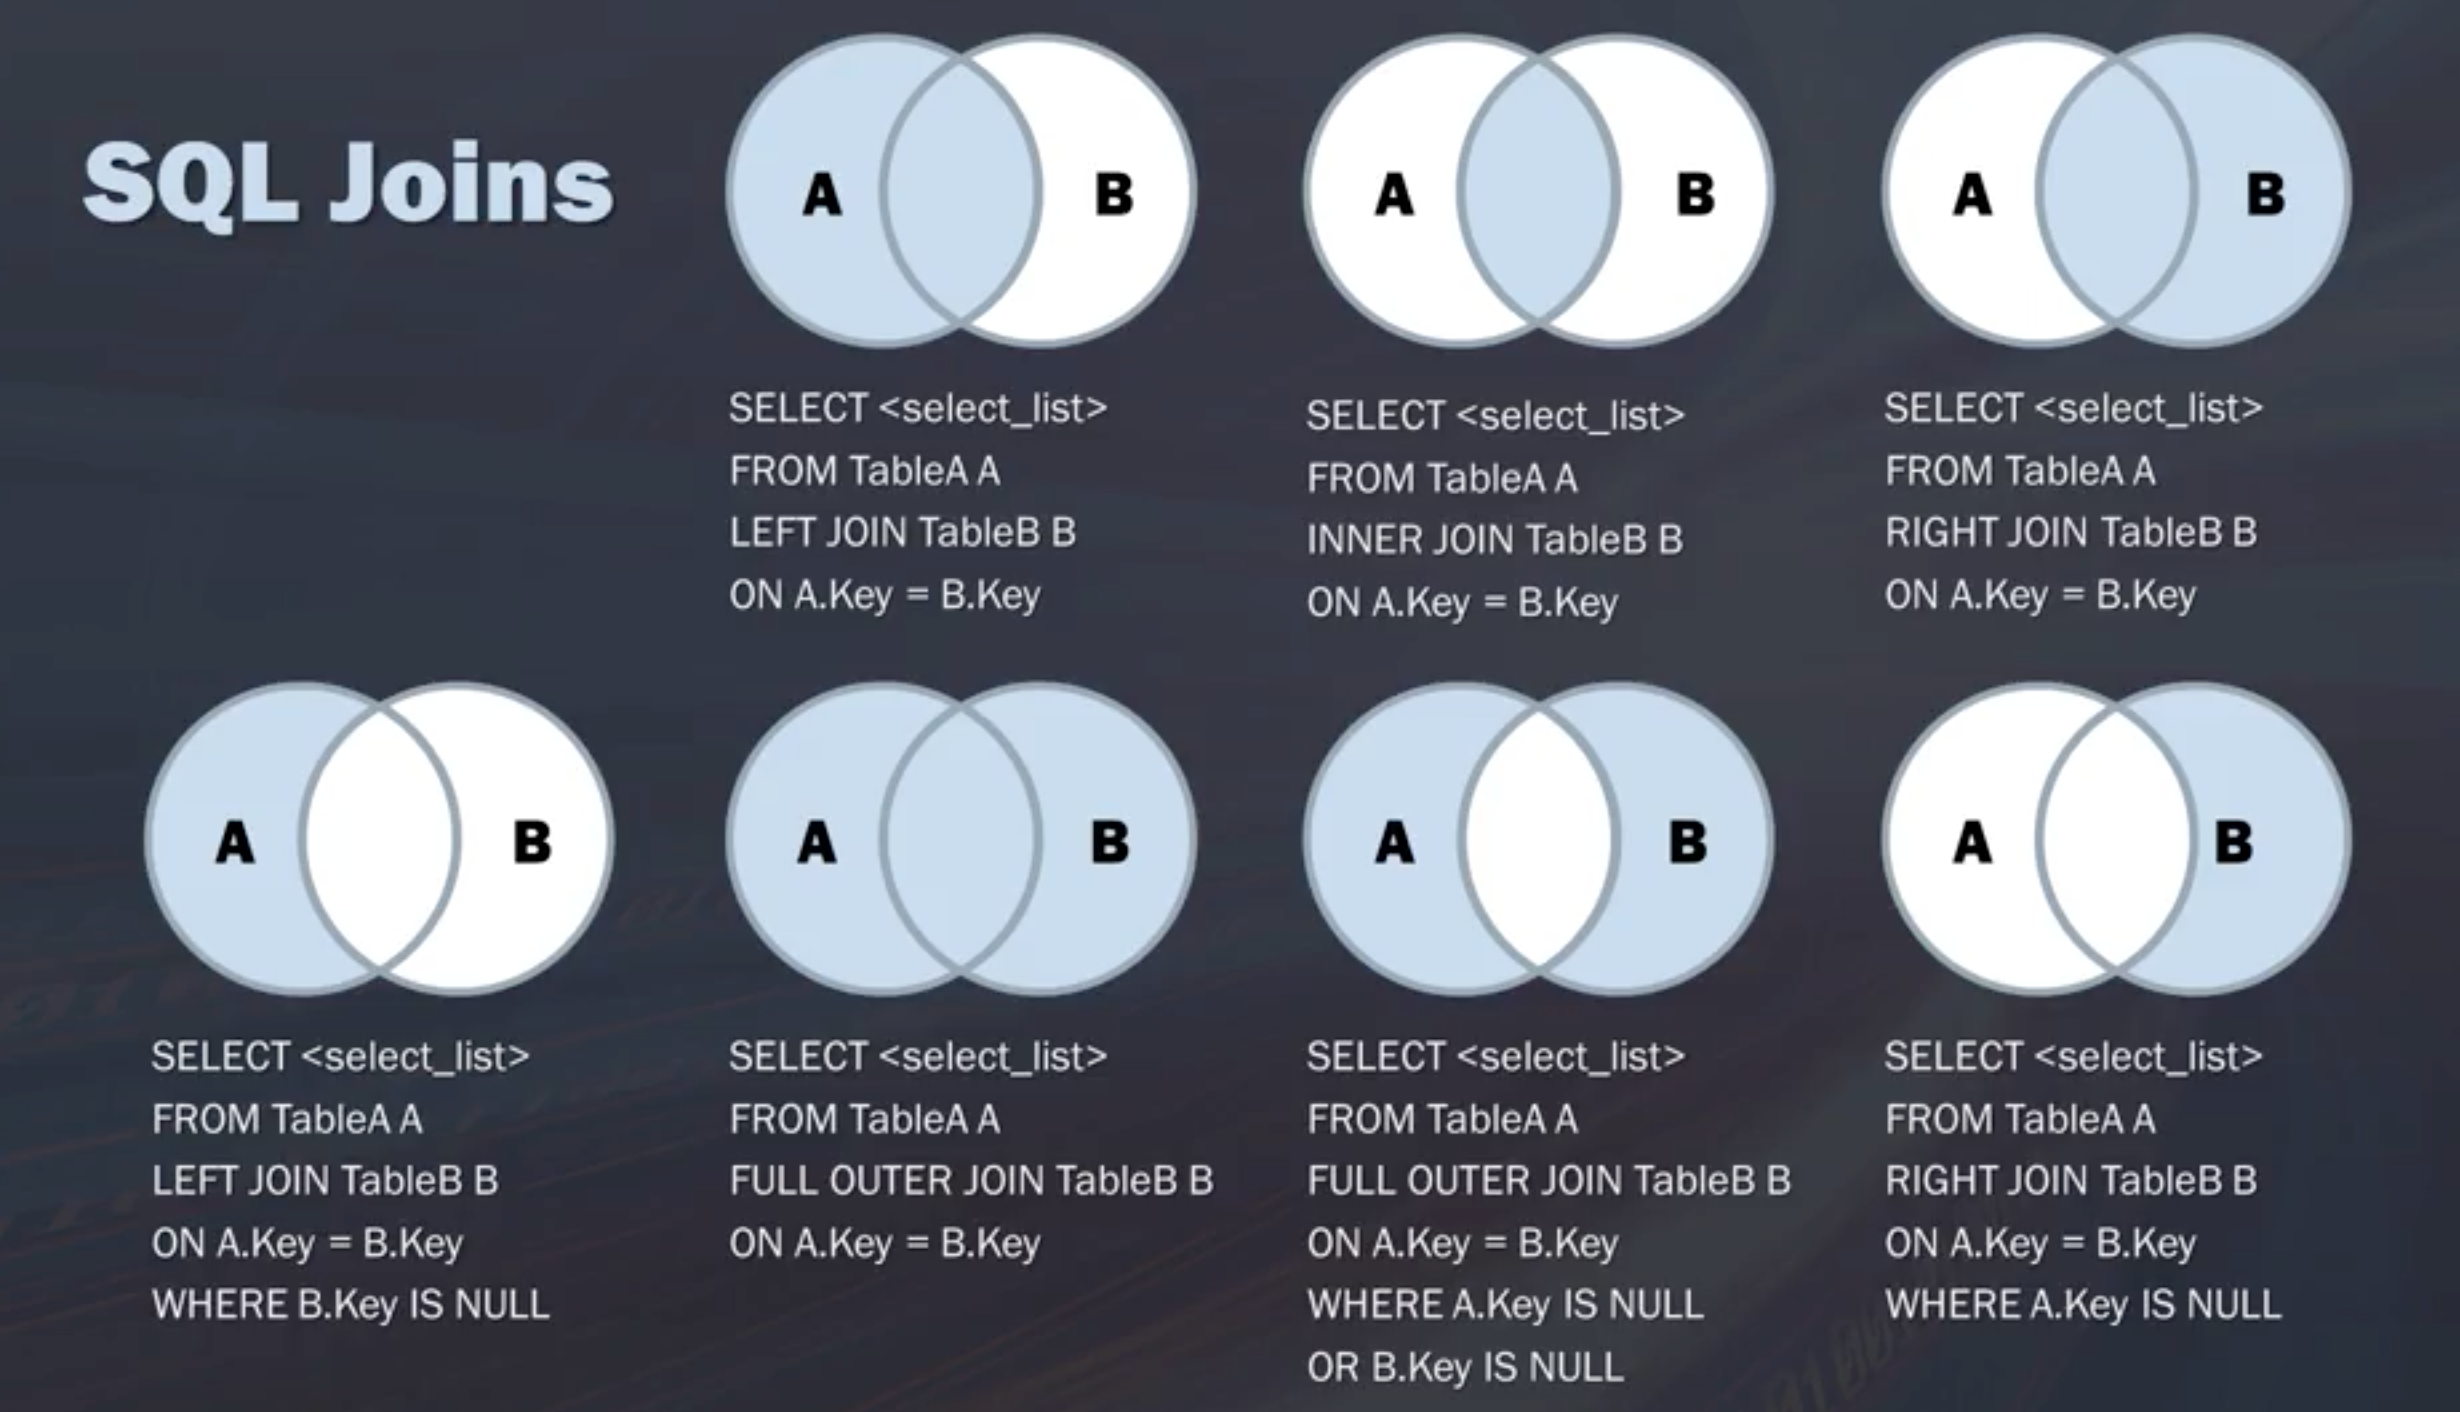
\includegraphics[width=0.80000\textwidth]{images/joindiagram.png}
\caption{}
\end{figure}

\begin{itemize}
\tightlist
\item
  Further Reading

  \begin{itemize}
  \tightlist
  \item
    \href{https://blog.modeanalytics.com/learning-python-sql/}{Thinking
    in SQL vs Thinking in Python}
  \item
    \href{https://blog.sqlauthority.com/2009/03/11/sql-server-difference-between-union-vs-union-all-optimal-performance-comparison/}{Difference
    Between Union and Union All - Optimal Performance Comparison}
  \end{itemize}
\end{itemize}

\chapter{Modifying and Analyzing Data with
SQL}\label{modifying-and-analyzing-data-with-sql}

\section{Text Strings}\label{text-strings}

\begin{itemize}
\tightlist
\item
  Concatenate or combine strings
\end{itemize}

SQL use the pipe or vertical bar key (\texttt{\textbar{}\textbar{}}) to
concatenate strings. The following example concatenates the company name
and the contact name. What it does are:

\begin{enumerate}
\def\labelenumi{\arabic{enumi}.}
\tightlist
\item
  use \texttt{SELECT} statement to pull the company name and contact
  name
\item
  concatenate these two together
\end{enumerate}

\begin{Shaded}
\begin{Highlighting}[]
\KeywordTok{SELECT}
\NormalTok{CompanyName, ContactName, CompanyName || }\StringTok{'  ( '} \NormalTok{|| ContactName || }\StringTok{' ) '}
\KeywordTok{FROM} \NormalTok{customers}
\end{Highlighting}
\end{Shaded}

It's important to know that the different relational database management
systems use different formats. SQL server, for example, uses the plus
sign (\texttt{+}) instead of a pipe (\texttt{\textbar{}\textbar{}}).

\begin{itemize}
\tightlist
\item
  Trim strings
\end{itemize}

With trimming function, you can either trim everything off the front and
the back, or you can just trim it from the right or left. To do this,
we're going to use the simple function called \texttt{TRIM}. We also
have \texttt{RTRIM} and \texttt{LTRIM}, for right trim and left trim
respectively.

In the following example, there are trailing spaces before and after the
string. The \texttt{TRIM} takes care of all of the trailing spaces which
is an easy way to clean up your data and will save you a lot of hassle
in the long run.

\begin{Shaded}
\begin{Highlighting}[]
\KeywordTok{SELECT} \FunctionTok{TRIM} \NormalTok{(}\OtherTok{"  You the best,      "}\NormalTok{)  }\KeywordTok{AS} \NormalTok{TrimmedString;}
\end{Highlighting}
\end{Shaded}

\begin{itemize}
\tightlist
\item
  Use the substring function
\end{itemize}

Substring returns the specified number of characters from a particular
position of a given string

\begin{longtable}[]{@{}ll@{}}
\toprule
First\_name & \texttt{substr(first\_name,\ 2,\ 3)}\tabularnewline
\midrule
\endhead
Alexander & lex\tabularnewline
Bruce & ruc\tabularnewline
David & avi\tabularnewline
Valli & all\tabularnewline
Diana & ian\tabularnewline
\bottomrule
\end{longtable}

In \texttt{substr(first\_name,\ 2,\ 3)}, the first one is string name,
the second one is string position, and the third is number of characters
to be returned.

\begin{Shaded}
\begin{Highlighting}[]
\KeywordTok{SELECT} \NormalTok{first_name, }\FunctionTok{SUBSTR}\NormalTok{(first_name, }\DecValTok{2}\NormalTok{, }\DecValTok{3}\NormalTok{)}
\KeywordTok{FROM} \NormalTok{employees}
\KeywordTok{WHERE} \NormalTok{department_id = }\DecValTok{60}\NormalTok{;}
\end{Highlighting}
\end{Shaded}

\begin{itemize}
\tightlist
\item
  Change the case of strings
\end{itemize}

This is an easy one : )

\begin{Shaded}
\begin{Highlighting}[]
\KeywordTok{SELECT} \FunctionTok{UPPER}\NormalTok{(column_name) }\KeywordTok{FROM} \NormalTok{table_name;}
\KeywordTok{SELECT} \FunctionTok{LOWER}\NormalTok{(column_name) }\KeywordTok{FROM} \NormalTok{table_name;}
\NormalTok{SLECT UCASE(column_name) }\KeywordTok{FROM} \NormalTok{table_name;}
\end{Highlighting}
\end{Shaded}

\section{Date and Time Strings}\label{date-and-time-strings}

Learning Objectives:

\begin{itemize}
\tightlist
\item
  Describe the complexities of adjusting date and time strings
\item
  Discuss the different formats in which dates and times are presented
\item
  List and describe the five different functions in SQL that can be used
  to manipulate data time strings
\end{itemize}

\bibliography{book.bib}

\backmatter
\printindex

\end{document}
